% $Id: cnrs-2001.tex,v 1.11 2001-06-18 08:16:56 geuzaine Exp $

\documentclass[a4]{seminar}

\usepackage{talks}

\typeout{}
\typeout{*******************************************************}
\typeout{* Do you want to include all the pictures? (you need}
\typeout{* to checkout the getdp-picts module at the same level}
\typeout{* as getdp for this)? (0/1)}
\typein[\bigpictures]
        {*******************************************************}

\fulltitle=0 % set to 1 to get full authors/affiliation on title pages

\begin{document}

%\talk{CNRS Grenoble June 20, 2001}
\talk{Software environment}

\begin{slide}

\slidepagestyle{none}

\begin{center}
\bigtitle{Benefits of an open software environment for the modeling of
          coupled electromagnetic problems}\\
\bigskip\bigskip
\mediumtitle{Christophe Geuzaine}\\
\bigskip
\smalltitle{Department of Electrical Engineering}\\
\smalltitle{Montefiore Institute B28, Sart Tilman Campus}\\
\smalltitle{University of Li�ge}\\
\smalltitle{B-4000 Li�ge (BELGIUM)}
\end{center}

\end{slide}

% Summary: With its strong mathematical foundations, the finite element
% method is an invaluable tool for the modeling of complex coupled
% physical problems that cannot be solved by analytical methods. Indeed,
% automatic mesh generation and mixed finite elements have tremendously
% widened its range of application, and call for a more general software
% implementation.
% The presentation will focus on such a generalization, called GetDP,
% which is freely available on the Internet for research in collaboration.
% After an overview of the general working philosophy of the software, the
% benefits it may bring for the modeling of magnetic problems (taking
% thermal, mechanical and circuit couplings into account) will be
% highlighted thanks to a couple of examples. Topics which could be
% studied in collaboration will then be presented, such as error
% estimation or the use of the software as a black box in higher level
% optimization packages.

% $Id: fem.tex,v 1.13 2001-07-20 16:51:52 geuzaine Exp $

% ---------------------------------------------------------------------------
\part{Introduction}
% ---------------------------------------------------------------------------

\begin{slide}

\slidepagestyle{none}

\begin{center}
\bigtitle{Introduction --- finite element methods}
\ifnum\fulltitle=1\par\bigskip\bigskip
\mediumtitle{Christophe Geuzaine}\\
\bigskip
\smalltitle{Department of Electrical Engineering}\\
\smalltitle{Montefiore Institute B28, Sart Tilman Campus}\\
\smalltitle{University of Li�ge}\\
\smalltitle{B-4000 Li�ge (BELGIUM)}
\fi
\end{center}

\end{slide}

% ---------------------------------------------------------------------------

\chapter{Coupled electromagnetic problems?}

\begin{slide}

Maxwell's equations, coupled with...

\begin{slideitemize}
\item Electric and electronic \emph{circuits} (power electronic supplies)
\item \emph{Mechanical} phenomena (force calculation, magnetostriction,
piezoelectricity, noise and vibrations)
\item \emph{Thermal} phenomena (thermal losses, induction heating, dielectric heating)
\item \emph{Fluid} dynamics (charged particles, magnetohydrodynamics)
\end{slideitemize}

\end{slide}

% ---------------------------------------------------------------------------

\chapter{Computational methods?}

\begin{slide}

\begin{slideitemize}
\item \emph{Analytic} models are difficult/impossible to apply to complex/coupled problems
\item \emph{Performance} (both floating point and visualization) of low end PCs is
exploding
\item Basic \emph{theory} of classic numerical methods (finite differences,
finite volumes, finite elements, integral methods) is well-known, and current
developments don't change the fundamental principles anymore
\end{slideitemize}

\end{slide}

% ---------------------------------------------------------------------------

\chapter{Finite element method (FEM)}

\begin{slide}

\begin{slideitemize}
\item The 1960s for mechanical problems (very large \emph{application range}
since the 1980s)
\item Strong \emph{mathematical foundations} (convergence, unicity)
\item Generalizations/re-interpretations (vanishing boundaries between finite
differences, finite elements and finite volumes, ...) call for a
\emph{single software implementation}
\end{slideitemize}

But FEM is not the magic/universal tool:
\begin{slideitemize}
\item Many conflicting/\emph{antinomic} issues (continuous vs. discontinuous
interpolation, conforming vs. non-conforming meshes, implicit vs. explicit
time integration, ...)
\item Generality has always an impact on \emph{efficiency}
\end{slideitemize}

\end{slide}

\begin{slide}

Based on a double \emph{discretization}:
\begin{slideitemize}
\item ``Replace'' the function spaces to which the fields belong (e.g.\
$\Hone{\Omega}$, $\Hcurl{\Omega}$, $\Hdiv{\Omega}$ or $\Ltwo{\Omega}$) by
\emph{finite dimensional subspaces}
\item ``Replace'' the domains on which these subspaces are defined by a
union of elementary geometrical elements of simple shapes (a ``\emph{mesh}''
or ``grid'')
\end{slideitemize}

\bigskip

\mybox{colbox}{0.98\textwidth}{
\begin{center}
FEM\\ $\Updownarrow$\\ the finite dimensional subspaces are built so that
their bases are \emph{piecewise} defined on the mesh
\end{center}
}

\end{slide}

\begin{slide}

One way to obtain a consistent Galerkin FEM formulation:
\begin{slideitemize}
\item Write a \emph{weak formulation} of the problem:

\begin{equation*}
\begin{cases}
L u = f \text{ in } \Omega \\
B u = g \text{ in } \Gamma 
\end{cases}
\Rightarrow\quad
\ivol[_\Omega]{u}{L^* v} - 
\ivol[_\Omega]{f}{v} + 
\int\limits_\Gamma Q_g(v) \, ds , 
\quad\forall v \in V(\Omega) 
\end{equation*}

% $L$ is a differential operator of order $n$ defined on $\Omega$
% 
% L^* is the adjoint of L:
%
% \ivol[_\Omega]{L u}{v} - \ivol[_\Omega]{u}{L^* v} = \int\limits_\Gamma Q(u,v) ds ,
%
% $Q$ is a bilinear function of $u$ and $v$ and in their derivatives up
% to the order $n-1$
%
% $Q_g$ is a linear form in $v$ which depends of $g$

\item Discretize with \emph{Whitney/mixed} elements $w_i$:
\begin{equation*}
\bar{u}, \bar{v} \in W(\Omega) , \quad
W(\Omega) = \text{span}\{w_i\} , \quad
W(\Omega) \subset V(\Omega)
\end{equation*}

% \bar{u} = \sum_{i} u_i w_i 

\end{slideitemize}

\end{slide}

\begin{slide}

\begin{slideitemize}
\item ``\emph{Nodal}'' elements for ``0-forms'' (\emph{continuous} scalar
fields like scalar potentials, temperature, pressure, ...)

\item ``\emph{Edge}'' elements for ``1-forms'' (vector fields with
\emph{continuous tangential components} across material interfaces, like
electric and magnetic fields, magnetic vector potential, ...)

\item ``\emph{Facet}'' elements for ``2-forms'' (vector fields with
\emph{continuous normal components} across material interfaces, like
magnetic flux density, current density, ...)

\item ``\emph{Volume}'' elements for ``3-forms'' (\emph{piecewise
continuous} scalar fields like charge density, heat source density, ...)

\end{slideitemize}

\end{slide}

% ---------------------------------------------------------------------------

\chapter{Controlling the error}

\begin{slide}

\emph{Error} on the solution of a discrete formulation:
\begin{slideitemize}
\item 
\emph{Hypotheses} in the continuous models (e.g.\ constitutive laws) 
\item 
\emph{Discretization} of the continuous model (finite dimensional spaces):
\begin{itemize}
\item 
Discretizing the \emph{geometry} (idealized geometry, meshed with a finite
number of elementary elements)
\item
Discretizing the \emph{fields} (locally approximated by polynomials of
finite order)
\end{itemize}
\end{slideitemize}

\end{slide}

\begin{slide}

\emph{Adaptation}: foresee/control the discretization error. Possible if
\begin{slideitemize}
\item
Knowledge of asymptotic \emph{error convergence}
\item
Availability of an error \emph{approximation} (if the exact value is known,
so is the exact solution!)
% the exact solution is also known!)
\end{slideitemize}

Goal: generate the best discrete function space possible 

Constraint: size of the function space or discretization error

Solution: modify (if possible, locally) the interpolation order
(\emph{$p$-refinement}) or the size of geometrical elements
(\emph{$h$-refinement})

\end{slide}

% ---------------------------------------------------------------------------

\chapter{Local and global errors}

\begin{slide}

If $u$ and $u'$ are the exact and approximate solutions on $\Omega$:
\begin{slideitemize}
\item
Elementary and global \emph{absolute} errors $e_i$ and $e$
\begin{equation*}
e_i^2 = \ivol[_{K_i}]{u'-u}{u'-u} \quad\text{and}\quad
e^2   = \ivol[_\Omega]{u'-u}{u'-u}
\end{equation*}
\item
Elementary and global \emph{relative} errors
\begin{equation*}
\varepsilon_i^2 = e_i^2 / n^2 \quad\text{and}\quad
\varepsilon^2   = e^2 / n^2 = \sum_{i=1}^N \varepsilon_i^2
\end{equation*}
\begin{equation*}
n^2 = \ivol[_\Omega]{u'+u}{u'+u}
\end{equation*}
\end{slideitemize}

\end{slide}

% ---------------------------------------------------------------------------

\chapter{Error convergence for elliptic problems}

\begin{slide}

\begin{slideitemize}
\item If $h_i$ and $p_i$ measure the size and polynomial degree of element
$K_i$: 
\begin{equation*}
\varepsilon_i = \Order\Big( \frac{1}{p_i} h_i^{\min(p_i,\gamma)} \Big) 
\end{equation*}
($\gamma$ depends on singularities of $u$)
\item
If \emph{uniform} error distribution (or no singularities):
\begin{equation*}
\varepsilon_i = \Order\Big( \frac{1}{p_i} h_i^{p_i} \Big) 
\end{equation*}
\end{slideitemize}

\end{slide}

% ---------------------------------------------------------------------------

\chapter{Error estimates through dual solutions}

\begin{slide}

\begin{slideitemize}
\item
Two \emph{dual} formulations, each being conform on one side of a Tonti diagram
\item
Error estimated through \emph{non fulfillment of the constitutive
relations}. For example:
\begin{equation*}
\varepsilon_i^\mu       = \frac{\Norm{\vec{b}-\mu\vec{h}}_{K_i}} 
                                {\Norm{\vec{b}+\mu\vec{h}}_\Omega} ,\quad
\varepsilon_i^\epsilon  = \frac{\Norm{\vec{d}-\epsilon\vec{e}}_{K_i}}
                                {\Norm{\vec{d}+\epsilon\vec{e}}_\Omega} \quad\text{and}\quad
\varepsilon_i^\sigma    = \frac{\Norm{\vec{j}-\sigma\vec{e}}_{K_i}}
                                {\Norm{\vec{j}+\sigma\vec{e}}_\Omega}
\end{equation*}
\item
\emph{Hypercirle theorem} implies upper bounds to the exact error for non
dissipative systems.
\item
For other systems, if mesh size sufficiently small, ...
\end{slideitemize}

\end{slide}

\begin{slide}

Example: convergence of global quantities (inductance and resistance) for
dual formulations

\centerline{
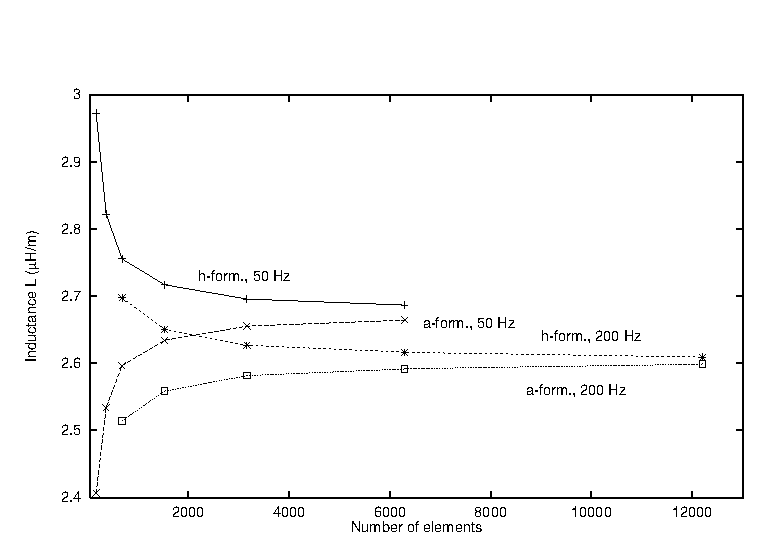
\includegraphics[width=11\semcm]{fig/IndL}
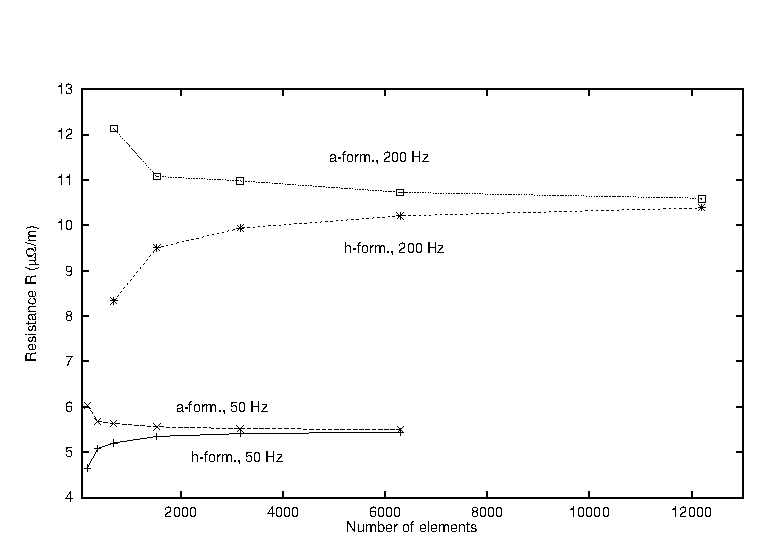
\includegraphics[width=11\semcm]{fig/IndR}
}

\end{slide}

\begin{slide}
\emph{Deterministic optimization of the global spaces}: minimize the number of
unknowns, while respecting a prescribed global error $\varepsilon_0$
\begin{equation*}
\min_{h_i',p_i'} \sum_{i=1}^N {p_i'}^3 (h_i/h_i')^3 
\quad\text{with}\quad
\varepsilon_0^2 =
\sum_{i=1}^N \varepsilon_i^2 \,
 \frac{p_i^2 \, {h_i'}^{2 p_i'}}{{p_i'}^2 \, h_i^{2 p_i}}
\end{equation*}

\begin{enumerate}
\item 
solve on $\mathcal{M}$;
\item 
create $\mathcal{M}'$ by \emph{$h$-adaptation} with a global constraint
$\alpha\varepsilon''$ ($\alpha>1$);
\item 
solve on $\mathcal{M}'$;
\item 
create $M''$ by \emph{$p$-adaptation} with the global constraint
$\varepsilon''$. Since the uniform error distribution was achieved on
$\mathcal{M}'$, this leads to the ideal convergence rate;
\item
solve on $\mathcal{M}''$.
\end{enumerate}
\end{slide}

\begin{slide}

Disadvantages of the dual approach:
\begin{slideitemize}
\item
Both dual formulations have to be solved (\emph{cost!})
\item
Implementation of one formulations usually (much) \emph{harder} than the
other
\end{slideitemize}

Solutions?
\begin{slideitemize}
\item
Projection techniques
\item
Generalize the software tools to tackle various formulations easily
\end{slideitemize}

\end{slide}

% $Id: getdp.tex,v 1.17 2001-07-17 23:27:44 geuzaine Exp $

\newcommand{\smallgetdp}[1]
   {\background{7\semcm}{4.2\semcm}{\scalebox{0.3}{\input{#1}}}}

% ---------------------------------------------------------------------------
\part{GetDP}
% ---------------------------------------------------------------------------

\begin{slide}

\slidepagestyle{none}

\begin{center}
\bigtitle{GetDP --- A general software environment for the treatment of
          discrete problems}\\
\ifnum\fulltitle=1\par\bigskip\bigskip
\mediumtitle{Patrick Dular and Christophe Geuzaine}\\
\bigskip
\smalltitle{Department of Electrical Engineering}\\
\smalltitle{Montefiore Institute B28, Sart Tilman Campus}\\
\smalltitle{University of Li�ge}\\
\smalltitle{B-4000 Li�ge (BELGIUM)}
\fi
\end{center}

\end{slide}

% ---------------------------------------------------------------------------

\chapter{An environment open to various couplings}

\begin{slide}

Any coupling between 
\begin{slideitemize}
\item \emph{Physical} problems (electromagnetic, thermal, mechanical, ...)
\item \emph{Numerical} methods (finite element methods, integral methods, ...)
\item \emph{Geometries} (1D, 2D, 3D)
\item \emph{Time} states (static, harmonic, transient)
\end{slideitemize}

How?
\begin{slideitemize}
\item Clear \emph{mathematical} definitions/structure
\item Directly transcribed into 10 interdependent \emph{objects}
\end{slideitemize}

\end{slide}

% ---------------------------------------------------------------------------

\chapter{Definition of discrete problems}

\begin{slide}

\begin{center}
Copy of the formal mathematical expression of problems in \emph{text data
files} (``\code{.pro} files'')
\end{center}

\begin{center}
\scalebox{0.54}{\input{fig/getdp-struct.tex}}
\end{center}

\end{slide}

\begin{slide}

\begin{center}
Particular data of a problem\\
\medskip
\scalebox{0.54}{\input{fig/getdp-struct-box.tex}}\\
\medskip
Method of resolution (``black box'')
\end{center}

\end{slide}

% ---------------------------------------------------------------------------

\smallgetdp{fig/getdp-struct-group.tex}

\chapter{\code{Group}: defining topological entities}

\begin{slide}

\mybox{colbox}{11\semcm}{
  \begin{slideitemize}
  \item Regions
  \item Functions on Regions (nodes, edges, edges of tree, ...)
  \end{slideitemize}
}

\bigskip
\begin{syntax}
Air = Region[1]; \CC{elementary group (linked with the mesh)}
Core = Region[2];
Omega = Region[\{Air, Core\}];
Nodes = NodesOf[Omega]; \CC{function group}
\end{syntax}

\end{slide}

% ---------------------------------------------------------------------------

\smallgetdp{fig/getdp-struct-function.tex}

\chapter{\code{Function}: defining expressions}

\begin{slide}

\mybox{colbox}{11\semcm}{
  \begin{slideitemize}
  \item Physical characteristics
  \item Time functions
  \item Various other functions (natural constraints, ...)
  \end{slideitemize}
}

\bigskip
\begin{syntax}
mu0 = 4.e-7*Pi; f = 50; \CC{constants}
mu[Air] = mu0; 
mu[Core] = mu0 + 1/(100+100*$1^6); \CC{argument ($1 <- b)}
TimeFct[] = Cos[2*Pi*f*$Time] * Exp[-$Time/0.012]; \CC{current value}
\end{syntax}

\end{slide}

% ---------------------------------------------------------------------------

\smallgetdp{fig/getdp-struct-constraint.tex}

\chapter{\code{Constraint}: specifying constraints}

\begin{slide}

\mybox{colbox}{11\semcm}{
  \begin{slideitemize}
  \item Boundary conditions (classical, connection)
  \item Initial conditions
  \item Topology of circuits with lumped elements
  \item Other constraints (on local and global quantities)
  \end{slideitemize}
}

\bigskip
\begin{syntax}
\{ Name Dirichlet; Type Assign; \CC{boundary conditions}
  Case \{ \{ Region Surface0; Value 0; \}
         \{ Region Surface1; Value 1; \} \}
\}
\end{syntax}

\end{slide}

\background{7\semcm}{-2.5\semcm}{\scalebox{0.65}{\begin{picture}(0,0)%
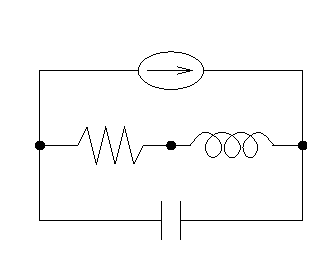
\includegraphics{getdp-rlccircuit}%
\end{picture}%
\setlength{\unitlength}{3947sp}%
%
\begingroup\makeatletter\ifx\SetFigFont\undefined%
\gdef\SetFigFont#1#2#3#4#5{%
  \reset@font\fontsize{#1}{#2pt}%
  \fontfamily{#3}\fontseries{#4}\fontshape{#5}%
  \selectfont}%
\fi\endgroup%
\begin{picture}(2387,1794)(1923,-4573)
\put(4310,-3856){\makebox(0,0)[lb]{\smash{\SetFigFont{10}{12.0}{\rmdefault}{\mddefault}{\updefault}{\color[rgb]{0,0,0}$2$}%
}}}
\put(3601,-3586){\makebox(0,0)[lb]{\smash{\SetFigFont{10}{12.0}{\rmdefault}{\mddefault}{\updefault}{\color[rgb]{0,0,0}$L_1$}%
}}}
\put(3076,-2944){\makebox(0,0)[lb]{\smash{\SetFigFont{10}{12.0}{\rmdefault}{\mddefault}{\updefault}{\color[rgb]{0,0,0}$E_1$}%
}}}
\put(2615,-3527){\makebox(0,0)[lb]{\smash{\SetFigFont{10}{12.0}{\rmdefault}{\mddefault}{\updefault}{\color[rgb]{0,0,0}$R_1$}%
}}}
\put(1923,-3869){\makebox(0,0)[lb]{\smash{\SetFigFont{10}{12.0}{\rmdefault}{\mddefault}{\updefault}{\color[rgb]{0,0,0}$1$}%
}}}
\put(3119,-3710){\makebox(0,0)[lb]{\smash{\SetFigFont{10}{12.0}{\rmdefault}{\mddefault}{\updefault}{\color[rgb]{0,0,0}$3$}%
}}}
\put(3086,-4138){\makebox(0,0)[lb]{\smash{\SetFigFont{10}{12.0}{\rmdefault}{\mddefault}{\updefault}{\color[rgb]{0,0,0}$C_1$}%
}}}
\end{picture}
}}

\begin{slide}

\begin{syntax}
\{ Name Current; Type Assign; \CC{constraints on global quantities}
  Case \{ 
    \{ Region Inductor1; Value 1000; TimeFunction TimeFct[]; \} 
  \} 
\}

\{ Name ElectricalCircuit; Type Network; \CC{circuit}
  Case Circuit1 \{ 
    \{ Region E1; Branch \{1,2\}; \}
    \{ Region R1; Branch \{1,3\}; \}
    \{ Region L1; Branch \{3,2\}; \}
    \{ Region C1; Branch \{1,2\}; \}
  \}
\}
\end{syntax}

\end{slide}


% ---------------------------------------------------------------------------

\smallgetdp{fig/getdp-struct-functionspace.tex}

\chapter{\code{FunctionSpace}: building function spaces}

\begin{slide}

\mybox{colbox}{11\semcm}{
  \begin{slideitemize}
  \item Various quantity types (0, 1, 2, 3-forms, scalar, vector)
  \item Various basis functions (associated with nodes, edges, facets,
  volumes) of various orders
  \item Coupling of fields and potentials ($\vec{t}$-$\omega$, $\vec{h}$-$\phi$,
  $\vec{a}$-$v$, ...)
  \item Definition of global quantities (fluxes, circulations: current,
  voltage, m.m.f., ...)
  \item Essential constraints (boundary and gauge conditions, ...)
  \end{slideitemize}
}

\rput(0.75\textwidth,4\semcm){\begin{picture}(0,0)%
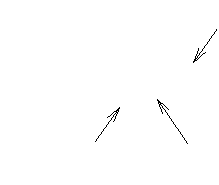
\includegraphics{getdp-sum}%
\end{picture}%
\setlength{\unitlength}{3947sp}%
%
\begingroup\makeatletter\ifx\SetFigFont\undefined%
\gdef\SetFigFont#1#2#3#4#5{%
  \reset@font\fontsize{#1}{#2pt}%
  \fontfamily{#3}\fontseries{#4}\fontshape{#5}%
  \selectfont}%
\fi\endgroup%
\begin{picture}(1742,1435)(2020,-4818)
\put(2020,-4668){\makebox(0,0)[lb]{\smash{\SetFigFont{10}{12.0}{\rmdefault}{\mddefault}{\updefault}{\color[rgb]{0,0,0}\small Geometrical}%
}}}
\put(2162,-4818){\makebox(0,0)[lb]{\smash{\SetFigFont{10}{12.0}{\rmdefault}{\mddefault}{\updefault}{\color[rgb]{0,0,0}\small entities}%
}}}
\put(3220,-4668){\makebox(0,0)[lb]{\smash{\SetFigFont{10}{12.0}{\rmdefault}{\mddefault}{\updefault}{\color[rgb]{0,0,0}\small Degrees of}%
}}}
\put(3321,-4817){\makebox(0,0)[lb]{\smash{\SetFigFont{10}{12.0}{\rmdefault}{\mddefault}{\updefault}{\color[rgb]{0,0,0}\small freedom}%
}}}
\put(3244,-3488){\makebox(0,0)[lb]{\smash{\SetFigFont{10}{12.0}{\rmdefault}{\mddefault}{\updefault}{\color[rgb]{0,0,0}\small Basis functions}%
}}}
\put(2176,-4036){\makebox(0,0)[lb]{\smash{\SetFigFont{10}{12.0}{\rmdefault}{\mddefault}{\updefault}{\color[rgb]{0,0,0}$f(\vec{x})=\sum_{i\in E}f_i w_i(\vec{x})$}%
}}}
\end{picture}
}

\end{slide}

\background{}{}{}

\begin{slide}

\begin{syntax}
\{ Name H1; Type Form0; \CC{discrete function space for H1}
  BasisFunction \{
    \{ Name wi; NameOfCoef fi; Function BF_Node; \CC{order 1}
      Support Omega; Entity NodesOf[All]; \}
    \{ Name wi2; NameOfCoef fi2; Function BF_Node_2E;  \CC{order 2}
      Support Omega; Entity EdgesOf[All]; \}
  \}
  Constraint \{
    \{ NameOfCoef fi; \CC{cf. 'Constraint'}
      EntityType NodesOf; NameOfConstraint Dirichlet; \}
    \{ NameOfCoef fi2;
      EntityType EdgesOf; NameOfConstraint Dirichlet2; \}
  \}
\}
\end{syntax}

\end{slide}


% ---------------------------------------------------------------------------

\smallgetdp{fig/getdp-struct-jacobian.tex}

\chapter{\code{Jacobian}: defining jacobian methods}

\begin{slide}

\mybox{colbox}{11\semcm}{
  \begin{slideitemize}
  \item Mapping from reference to real space 
  \item Geometrical transformations (axisymmetric transformation, infinite
  domains, ...)
  \end{slideitemize}
}

\bigskip
\begin{syntax}
\{ Name Jacobian1;
  Case \{ \CC{piece-wise defined on groups}
    \{ Region OmegaInf; Jacobian VolSphShell\{Rint, Rext\}; \}
    \{ Region OmegaAxi; Jacobian VolAxi; \}
    \{ Region All; Jacobian Vol; \}
  \}
\}
\end{syntax}

\end{slide}

% ---------------------------------------------------------------------------

\smallgetdp{fig/getdp-struct-integration.tex}

\chapter{\code{Integration}: defining integration methods}

\begin{slide}

\bigskip
\bigskip
\mybox{colbox}{11\semcm}{
  \begin{slideitemize}
  \item Various numeric and analytic integration methods
  \item Criterion-based selection
  \end{slideitemize}
}

\bigskip
\bigskip
\begin{syntax}
\{ Name Integration1; Criterion Test[]; \CC{combination of methods}
  Case \{ 
    \{ Type Gauss;
      Case \{ \{ GeoElement Triangle; NumberOfPoints 12; \}
             \{ GeoElement Tetrahedron; NumberOfPoints 15; \} \} \}
    \{ Type Analytic; \}
  \} 
\}
\end{syntax}

\end{slide}

% ---------------------------------------------------------------------------

\smallgetdp{fig/getdp-struct-formulation.tex}

\chapter{\code{Formulation}: building equations}

\begin{slide}

\mybox{colbox}{11\semcm}{
  \begin{slideitemize}
  \item Various formulation types: FEM, BEM, circuit equations, ...
  \item Symbolic expression of equations: volume and surface integral
  terms, collocation
  \item Involves local, global and integral quantities based on function
  spaces
  \end{slideitemize}
}

\begin{syntax}
Equation \{
  Galerkin \{ DtDt [ epsilon[] * Dof\{e\} , \{e\} ]; ... \}
  Galerkin \{ [ 1/mu[] * Dof\{Curl e\} , \{Curl e\} ]; ... \}
\}
\end{syntax}

\rput(0.8\textwidth,6\semcm)
     {$\partial_t^2\ivol{\epsilon\vec{e}}{\vec{e}'} + 
       \ivol{\mu^{-1}\Curl{\vec{e}}}{\Curl{\vec{e}'}}=0$}

\end{slide}

% ---------------------------------------------------------------------------

\smallgetdp{fig/getdp-struct-resolution.tex}

\chapter{\code{Resolution}: solving systems of equations}

\begin{slide}

\mybox{colbox}{10\semcm}{
  \begin{slideitemize}
  \item Description of a sequence of operations
  \item Time loops (with time step adaptation)
  \item Nonlinear iterative loops (e.g.\ fixed point or Newton-Raphson methods)
  \item Coupled problems (e.g.\ magneto-thermal coupling)
  \item Linking of various resolution steps (e.g.\ pre-computation of source
  fields) 
  \end{slideitemize}
}

\rput(0.8\textwidth,4\semcm){\parbox{12\semcm}{
\begin{syntax}
Operation\{\\
\hspace*{1em}InitSolution[A];\\
\hspace*{1em}TimeLoopTheta[tmin,tmax,dt,1]\{\\
\hspace*{2em}Generate[A]; Solve[A];\\
\hspace*{2em}If[Save[]]\{ SaveSolution[A]; \}\\
\hspace*{1em}\}\\
\}
\end{syntax}
}}

\end{slide}

% ---------------------------------------------------------------------------

\smallgetdp{fig/getdp-struct-postprocessing.tex}

\chapter{\code{PostProcessing}: exploiting computational data}

\begin{slide}

\mybox{colbox}{11\semcm}{
  \begin{slideitemize}
  \item ``Front-end'' to computational data
  \item Piece-wise definition of any quantity of interest
  \item Local or integral evaluation
  \end{slideitemize}
}

\bigskip
\begin{syntax}
Quantity \{
  \{ Name FluxDensity;
    Value \{ Local \{ [ -mu[]*\{Grad phi\} ]; In Omega; \}
            Local \{ [ -\{dGreen\} ]; In BEM; \} \}
\}
\end{syntax}


\end{slide}

% ---------------------------------------------------------------------------

\smallgetdp{fig/getdp-struct-postoperation.tex}

\chapter{\code{PostOperation}: exporting results}

\begin{slide}

\mybox{colbox}{11\semcm}{
  \begin{slideitemize}
  \item Evaluation of post-processing quantities (e.g.\ maps, sections,
  local or global evaluation, ...)
  \item Operations on post-processing quantities (sorting, smoothing,
  adaptation, ...) 
  \item Various output formats (e.g.\ space or time oriented, text, binary,
  ...) 
  \end{slideitemize}
}

\bigskip
\begin{syntax}
Print[ FluxDensity, OnElementsOf Omega, File "b.pos", Format Gmsh ];
Print[ FluxDensity, OnLine \{\{0,0,0\}\{1,0,0\}\} \{100\}, File "b.txt" ];
\end{syntax}

\end{slide}


\background{}{}{}


% $Id: examples.tex,v 1.5 2001-06-15 07:38:53 geuzaine Exp $

%
% WARNING:
%
% If \bigpictures is set to 1, the pictures must have been checked out
% (cvs module name is getdp-picts) in the ../../../getdp-picts directory.
%
% ---------------------------------------------------------------------------

\begin{slide}

\slidepagestyle{none}

\begin{center}
\bigtitle{Examples}\\
\ifnum\fulltitle=1\par\bigskip\bigskip
\mediumtitle{Patrick Dular and Christophe Geuzaine}\\
\bigskip
\smalltitle{Department of Electrical Engineering}\\
\smalltitle{Montefiore Institute B28, Sart Tilman Campus}\\
\smalltitle{University of Li�ge}\\
\smalltitle{B-4000 Li�ge (BELGIUM)}
\fi
\end{center}

\end{slide}

% ---------------------------------------------------------------------------
\part{GetDP/Gmsh examples}
% ---------------------------------------------------------------------------

\chapter{Magnetostatics}

\ifnum\bigpictures=1
\ifx\pdfoutput\undefined

\begin{slide}

\begin{center}
\includegraphics[width=0.38\textwidth]{getdp-picts/ind1}%
\includegraphics[width=0.38\textwidth]{getdp-picts/ind2}

\includegraphics[width=0.38\textwidth]{getdp-picts/ind3}%
\includegraphics[width=0.38\textwidth]{getdp-picts/ind4}
\end{center}

\end{slide}

\fi
\fi

\begin{slide}

\mybox{colbox}{\textwidth}{
\begin{equation*}
\Curl{\vec{h}} = \vec{j} ,\quad
\Div{\vec{b}} = 0 \quad\text{and}\quad
\vec{b} = \mu \vec{h} + \mu_0 \vec{h}_m 
\end{equation*}
\begin{equation*}
\begin{split}
\xymatrix{
 \color{colpos}\phi    \ar@{->}[r]^-{\GradSymb_h}  &
 \vec{h} \ar@{->}[r]^-{\CurlSymb_h} \ar@{<->}[d]^{\mu} &
 \vec{j} \ar@{->}[r]^-{\DivSymb_h}   &
 0 \\
 0       \ar@{<-}[r]^-{\DivSymb_e}&
 \vec{b} \ar@{<-}[r]^-{\CurlSymb_e}&
 \color{colpos}\vec{a} 
}
\end{split}
\end{equation*}
}

\begin{slideitemize}
\item Weak form of Gauss law: 
\begin{equation*}
%\ivol{\Div{\vec{b}}}{\phi'} = 0 \Rightarrow
\ivol{\vec{b}}{\Grad{\phi'}} + \isur{\psca{\vec{n}}{\vec{b}}}{\phi'} 
= 0
\quad \forall\phi'\in\Hone[_0]{\Omega}
\end{equation*}

\item Weak form of Ampere's law:
\begin{equation*}
%\ivol{\Curl{\vec{h}}}{\vec{a}'} = \ivol{\vec{j}}{\vec{a}'} \Rightarrow
\ivol{\vec{h}}{\Curl{\vec{a}'}} + \isur{\pvec{\vec{n}}{\vec{h}}}{\vec{a}'}
= \ivol{\vec{j}}{\vec{a}'} 
\quad \forall\vec{a}'\in\Hcurl[_0]{\Omega}
\end{equation*}

\end{slideitemize}

\end{slide}

% ---------------------------------------------------------------------------

\chapter{Magnetostatics: $\vec{b}$-conform}

\begin{slide}

\mybox{colbox}{\textwidth}{
\begin{center}
\emph{Vector potential} formulation
\begin{equation*}
\vec{b} = \Curl{\vec{a}}
\end{equation*}
\end{center}
}

\begin{center}
$\Downarrow$\\
Weak form of Amp�re's law\\
$\Downarrow$\\
$\displaystyle\ivol{\mu^{-1}\Curl{\vec{a}}}{\Curl{\vec{a}'}} 
= \ivol{\vec{j}}{\vec{a}'} ,
\quad\forall\vec{a}'\in\Hcurl[_0]{\Omega}$
\end{center}

\bigskip
NB: gauge for $\vec{a}$, ...

\end{slide}

\ifnum\bigpictures=1
\ifx\pdfoutput\undefined
\background{7\semcm}{0\semcm}{\includegraphics[width=0.38\textwidth]{getdp-picts/ind1}}
\fi\fi

\begin{slide}

\begin{smallsyntax}
Group \{
  Core = 1; Inductor = 2; SkinInductor = 3, Air = 4;
  Omega = Region[\{Core, Inductor, Air\}];
\}
Function \{
  mu0 = 4.e-7 * Pi; mur = 1000;
  mu[ Core ] = mur * mu0;
  mu[ Region[\{Air, Inductor\}] ] = mu0;
  j[ Inductor ] = ...; //to be defined
\}
Constraint \{
  \{ Name a; 
    Case \{ 
      \{ Region CL_a0; Value 0; \}
    \}
  \}
\}
\end{smallsyntax}

\end{slide}

\background{}{}{}

\begin{slide}

\begin{smallsyntax}
FunctionSpace \{
  \{ Name Hcurl; Type Form1; \CC{vector potential}
    BasisFunction \{
      \{ Name se;  NameOfCoef ae; Function BF_Edge; Support Omega; 
        Entity EdgesOf[All]; \} \CC{associated with the edges of the mesh}
    \}
    Constraint \{ \CC{essential constraint + gauge (unicity)}
      \{ NameOfCoef ae;  EntityType EdgesOf ; NameOfConstraint a; \}
      \{ NameOfCoef ae;  EntityType EdgesOfTreeIn ; EntitySubType StartingOn;
        NameOfConstraint Gauge ; \}
    \}
  \}
\}
\end{smallsyntax}

\end{slide}

\begin{slide}

\begin{smallsyntax}
Formulation \{
  \{ Name MagSta_a; Type FemEquation;
    Quantity \{ 
      \{ Name a ; Type Local; NameOfSpace Hcurl; \}
    \}
    Equation \{
      Galerkin \{ [ 1/mu[] * Dof\{Curl a\} , \{Curl a\} ]; 
                 In Omega; Integration I1; Jacobian JVol; \}
      Galerkin \{ [ -j[] , \{a\} ]; 
                 In Inductor; Integration I1; Jacobian JVol; \}
    \}
  \}
\}
\end{smallsyntax}

\end{slide}

\begin{slide}

\begin{smallsyntax}
Resolution \{
  \{ Name MagSta_a;
    System \{
      \{ Name A; NameOfFormulation MagSta_a; \}
    \}
    Operation \{ Generate A; Solve A; SaveSolution A; \}
  \}
\}
PostProcessing \{
  \{ Name test; NameOfFormulation MagSta_a;
    Quantity \{
      \{ Name a; Value \{ Local\{ [ \{a\} ]; In Omega; \} \} \}
      \{ Name normb; Value \{ Local\{ [ Norm[\{d a\}] ]; Omega; \} \} \}
    \}
  \}
\}
\end{smallsyntax}

\end{slide}

\begin{slide}

Magnetodynamics?

Additional term in the formulation: 

\begin{smallsyntax}
      Galerkin \{ DtDof [ sigma[] * Dof\{a\} , \{a\} ]; 
                 In Core; Integration I1; Jacobian JVol; \}   
\end{smallsyntax}

New resolution:
\begin{smallsyntax}
  \{ Name MagDyn_a_t; \CC{time domain}
    System \{
      \{ Name A; NameOfFormulation MagDyn_a; \}
    \}
    Operation \{ 
      InitSolution[A]
      TimeLoopTheta[0,20/50,0.1/50,1]\{
        Generate[A]; Solve[A]; SaveSolution[A];
      \}
    \}
  \}
\end{smallsyntax}


\end{slide}

% ---------------------------------------------------------------------------

\chapter{Magnetostatics: $\vec{h}$-conform}

\begin{slide}

\mybox{colbox}{\textwidth}{
\begin{center}
\emph{Magnetic field conform} formulation
\begin{equation*}
\vec{h} = \vec{h}_s+\vec{h}_r ,\quad\text{with}\quad
\Curl{\vec{h}_s} = \vec{j}     \quad\text{and}\quad
\vec{h}_r = -\Grad{\phi}
\end{equation*}
\end{center}
}

\begin{center}
$\Downarrow$\\
Weak form of Gauss law\\
$\Downarrow$\\
$\displaystyle\ivol{\mu(-\Grad{\phi}+\vec{h}_s)}{\Grad{\phi'}} 
= 0 ,
\quad \forall\phi'\in\Hone[_0]{\Omega}$
\end{center}

\bigskip
NB: choice of source field $\vec{h}_s$, treatment of multiply connected
$\Omega$, ...

\end{slide}

\begin{slide}

\begin{smallsyntax}
FunctionSpace \{
  \{ Name H1; Type Form0; \CC{scalar potential}
    BasisFunction \{
      \{ Name sn; NameOfCoef phin; Function BF_Node; Support Omega; 
        Entity NodesOf[All]; \} \CC{associated with the nodes of Omega}
    \}
    Constraint \{ \CC{essential constraint}
      \{ NameOfCoef phin; EntityType NodesOf; NameOfConstraint phi; \}
    \}
  \}
\}
\end{smallsyntax}

\end{slide}

\begin{slide}

\begin{smallsyntax}
Formulation \{
  \{ Name MagSta_phi; Type FemEquation;
    Quantity \{
      \{ Name phi; Type Local; NameOfSpace H1; \}
      \{ Name hs; Type Local; NameOfSpace Hcurl_s; \}  \CC{a little patience...}
    \}
    Equation \{
      Galerkin \{ [ mu[] * \{hs\} , \{Grad phi\} ];
                 In Omega; Integration I1; Jacobian JVol;  \}
      Galerkin \{ [ mu[] * Dof\{Grad phi\} , \{Grad phi\} ]; 
                 In Omega; Integration I1; Jacobian JVol;  \}
    \}
  \}
\}

\end{smallsyntax}

\end{slide}

\begin{slide}

\begin{smallsyntax}
FunctionSpace \{
  \{ Name Hcurl_s; Type Form1; \CC{space for the source field}
    BasisFunction \{
      \{ Name se; NameOfCoef he; Function BF_Edge; Support Inductor; 
        Entity EdgesOf[All, Not SkinInductor]; \}
      \{ Name sc; NameOfCoef Ic; Function BF_GradGroupOfNodes; 
        Support Transition; Entity GroupsOfNodesOf[Cut]; \}
      \{ Name sc; NameOfCoef Icc; Function BF_GroupOfEdges; 
        Support Inductor; Entity ...; \}
    \}
    Constraint \{
      \{ NameOfCoef he; EntityType EdgesOfTreeIn; EntitySubType StartingOn;
        NameOfConstraint Gauge; \}
      \{ NameOfCoef Ic;  EntityType GroupsOfNodesOf; NameOfConstraint I; \}
      \{ NameOfCoef Icc; EntityType GroupsOfNodesOf; NameOfConstraint I; \}
    \}
  \}
\}
\end{smallsyntax}

%... -> GroupsOfEdgesOf[Cut, InSupport ElementsOf[SkinInductor, OnOneSideOf Cut] ]

\end{slide}

% ---------------------------------------------------------------------------

\chapter{Magneto-thermal coupling}

\begin{slide}
....
\end{slide}

% ---------------------------------------------------------------------------

\background{}{}{}

\ifnum\bigpictures=1
\ifx\pdfoutput\undefined

\chapter{Other examples...}

\begin{slide}

\begin{center}
\includegraphics[width=\textwidth]{getdp-picts/antenna1}
\includegraphics[width=\textwidth]{getdp-picts/antenna3}
\includegraphics[width=\textwidth]{getdp-picts/antenna2}
\includegraphics[height=\textheight]{getdp-picts/indheat}
\includegraphics[angle=-90,width=\textwidth]{getdp-picts/line220kv}
\includegraphics[height=\textheight]{getdp-picts/magnet}
\includegraphics[height=\textheight]{getdp-picts/motoras}
\includegraphics[width=\textwidth]{getdp-picts/f16a}
\includegraphics[width=\textwidth]{getdp-picts/f16b}

\hspace*{-0.2\textwidth}%
\includegraphics[width=0.5\textwidth]{getdp-picts/p20induc2}\hspace*{-0.2\textwidth}
\includegraphics[width=0.5\textwidth]{getdp-picts/p20}\hspace*{-0.2\textwidth}%
\includegraphics[width=0.5\textwidth]{getdp-picts/p20ada}\hspace*{-0.2\textwidth}%

piezo-electricity, magnetostriction, non-homogeneous waveguides, photonic
cristals, electromagnetic shielding, dielectric heating, ...

\end{center}



\end{slide}

\else

\fi
\fi

% $Id: gmsh.tex,v 1.15 2002-09-06 16:24:02 geuzaine Exp $

% ---------------------------------------------------------------------------
\part{Gmsh}
% ---------------------------------------------------------------------------

\begin{slide}

\slidepagestyle{none}

\begin{center}
\bigtitle{Gmsh --- Geometry, mesh, solver integration
          and visualization}\\
\ifnum\fulltitle=1\par\bigskip\bigskip
\begin{minipage}{0.5\textwidth}\center
\mediumtitle{Christophe Geuzaine}\\
\bigskip
\smalltitle{Applied and Computational Mathematics}\\
\smalltitle{California Institute of Technology}\\
\smalltitle{Pasadena, CA 91125 (USA)}
\end{minipage}%
\begin{minipage}{0.5\textwidth}\center
\mediumtitle{Jean-Fran�ois Remacle}\\
\bigskip
\smalltitle{Scientific Computation Research Center}\\
\smalltitle{Rensselaer Polytechnic Insitute}\\
\smalltitle{Troy, NY 12180 (USA)}
\end{minipage}
\fi
\end{center}

\end{slide}

% ---------------------------------------------------------------------------

\chapter{Finite element methods in practice}

\begin{slide}

Four main steps:
\begin{slideitemize}
\item \emph{Geometry}: CAD description
\item \emph{Mesh}: structured or unstructured mesh generator
\item \emph{Solver}: GetDP :-)
\item \emph{Post-processing}: visualization (2D and 3D)
\end{slideitemize}

Most of the time necessary to solve a problem is \emph{not} spent in the
solver step!

\end{slide}

% ---------------------------------------------------------------------------

\chapter{Geometry description}

\begin{slide}

Bottom-up definition:
\begin{slideitemize}
\item \emph{Points}
\item Oriented \emph{curves} (segments, circles, ellipses, splines, etc.)
\item Oriented \emph{surfaces} (plane, ruled, etc.)
\item \emph{Volumes}
\end{slideitemize}

Parametrization:
\begin{slideitemize}
\item Dedicated \emph{language}
\item \emph{Scripting} possibilities (loops, tests, arrays of variables,
etc.)
\end{slideitemize}

%For complex models, a top-down approach (e.g.\ Constructive Solid Geometry)
%may be better.

\end{slide}

% ---------------------------------------------------------------------------

\chapter{Mesh generation}

\begin{slide}

\begin{slideitemize}
\item \emph{Structured} (transfinite, elliptic, hyperbolic)
\item \emph{Unstructured} (Delaunay triangles/tetrahedra)
\begin{enumerate}
\item 
Mesh of a box including the convex polygon/polyhedron resulting from
curves/surfaces discretization
\item
Initial mesh by insertion of curves/surfaces nodes by the Bowyer algorithm
\item 
Boundary restoration to force presence of all edges/faces
\item 
Suppression of unwanted triangles/tetrahedra
\item
New node insertions by the Bowyer algorithm until the characteristic size of
each simplex $\leq$ characteristic length field evaluated at the center of
its circumscribed circle/sphere.
\item
Mesh post-processing and quality enforcement by node relocation and edge
swapping
\end{enumerate}
\end{slideitemize}

\end{slide}

% ---------------------------------------------------------------------------

\chapter{Solver integration}

\begin{slide}

\begin{minipage}{0.45\textwidth}
\emph{Batch}:
\begin{slideitemize}
\item Advanced users
\item No graphic overhead
\item Easily scriptable
\end{slideitemize}
For complex problems
\end{minipage}%
\begin{minipage}{0.1\textwidth}
vs.
\end{minipage}%
\begin{minipage}{0.45\textwidth}
\emph{Interactive}:
\begin{slideitemize}
\item Smoother learning curve
\item Better integration
\item Faster for testing
\end{slideitemize}
For testing/learning
\end{minipage}%

\bigskip\bigskip
\begin{center}
Solvers should provide \emph{both}
\end{center}

\end{slide}

\begin{slide}

Example: integration of GetDP
\begin{slideitemize}
\item \emph{High level (system calls)}: commercial applications (Matlab,
Mathematica, ...), shell scripts (bash, Perl, Python, ...), other
programming languages (C, C++, ...)
\item \emph{Medium level (sockets)}: customizable applications (Gmsh, ...),
shell scripts (Perl, Python, ...), other programming languages (C, C++, ...)
\item \emph{Low level (source code)}: programming languages (C, C++, ...)
\end{slideitemize}

\end{slide}

% ---------------------------------------------------------------------------

\chapter{Post-processing}

\begin{slide}

\begin{slideitemize}
\item \emph{Multiple views}, manipulated globally or individually
\item \emph{Scalar} views displayed by iso-value curves or color maps
\item \emph{Vector} and \emph{tensor} views displayed with 3D arrows or
displacement maps
\item Interactive \emph{functions} including offsets, elevation, interactive
color map and range modification, interactive animation, etc.
\item All functions are \emph{scriptable} (animation, movement, ...)
\item Various \emph{output formats} (bitmap or vector)
\item \emph{Modular} (plug-in mechanism)
\end{slideitemize}

\end{slide}

% ---------------------------------------------------------------------------

\ifnum\bigpictures=1

\chapter{Some examples}

\begin{slide}

\begin{center}
\includegraphics[width=\textwidth]{getdp-picts/f16a.jpg}
\includegraphics[width=\textwidth]{getdp-picts/shoulder3}
\includegraphics[width=\textwidth]{getdp-picts/shoulder6}
\includegraphics[width=\textwidth]{getdp-picts/magnetron1}
\includegraphics[width=\textwidth]{getdp-picts/magnetron3}
\includegraphics[width=\textwidth]{getdp-picts/magnetron4}
\includegraphics[width=0.75\textwidth]{getdp-picts/tresse2}
\includegraphics[width=\textwidth]{getdp-picts/breaker}
\end{center}

\end{slide}

\fi

% ---------------------------------------------------------------------------


% $Id: conclusion.tex,v 1.4 2001-06-17 21:07:00 geuzaine Exp $

% ---------------------------------------------------------------------------
\part{Conclusions}
% ---------------------------------------------------------------------------

\begin{slide}

\slidepagestyle{none}

\begin{center}
\bigtitle{Conclusions}
\end{center}

\end{slide}

% ---------------------------------------------------------------------------

\chapter{Conclusions}

\begin{slide}

\begin{slideitemize}
\item Structured and concise software environment
\begin{itemize}
\item Numerical modeling of physical problems (but \emph{no physics inside the code}!)
\item User-friendly \emph{language for the definition of methods and problems}
\item Convenient for \emph{research}, \emph{application} or \emph{teaching}
\item Shared for collaboration (\emph{freely available} on the Internet,
documentation, mailing lists)
\end{itemize}
\end{slideitemize}

\end{slide}

\begin{slide}

\begin{slideitemize}
\item Adapted for stage-by-stage use
\begin{itemize}
\item \emph{From 1D to 3D} models
\item \emph{From linear to nonlinear} problems
\item \emph{From static to dynamic} problems
\item \emph{From single} physical or numerical \emph{models to coupled} ones
\end{itemize}
\item Open to new developments
\begin{itemize}
\item Open for adding \emph{new functionalities} in a progressive way
\item \emph{Interactive use} possible through Gmsh or home-made application
\item \emph{Integration} into higher level optimization packages
\end{itemize}

\end{slideitemize}

\end{slide}


\end{document}

